\newcommand{\texCommand}[1]{\texttt{\textbackslash{#1}}}%

\newcommand{\exemplo}[1]{%
\vspace{\baselineskip}%
\noindent\fbox{\begin{minipage}{\textwidth}#1\end{minipage}}%
\\\vspace{\baselineskip}}%

\newcommand{\exemploVerbatim}[1]{%
\vspace{\baselineskip}%
\noindent\fbox{\begin{minipage}{\textwidth}%
#1\end{minipage}}%
\\\vspace{\baselineskip}}%

\par Este capítulo introduz e explica todos os conceitos teóricos necessários para o entendimento do projeto proposto. Explica o que é biometria, o que são sistemas biométricos, o que é processamento de imagens no domínio espacial, processamento morfológico de imagens, filtragem em imagens e sistemas de reconhecimento de íris.

%%%%%%%%%%%%%%%%%%%%%%%%%%%%%%%%%%%%%%%%%%%%%%%%%%%%%%%%%%%%%%%%%%%%%%%%%%%%%%%%
%%%%%%%%%%%%%%%%%%%%%%%%%%%%%%%%%%%%%%%%%%%%%%%%%%%%%%%%%%%%%%%%%%%%%%%%%%%%%%%%
%%%%%%%%%%%%%%%%%%%%%%%%%%%%%%%%%%%%%%%%%%%%%%%%%%%%%%%%%%%%%%%%%%%%%%%%%%%%%%%%
\section{Biometria} \label{sec:fundamentacao:biometria}

\par Biometria são medidas físicas ou comportamentais que identificam um indivíduo unicamente \cite{li2009encyclopedia}. Nas últimas décadas, com os avanços das tecnologias, foi possível usar essas medidas biométricas em sistemas de autenticação \cite{wayman2005biometric}. 

\par As Subseções \ref{sec:fundamentacao:biometria:caracteristicas} e \ref{sec:fundamentacao:biometria:criterios} explicam quais as características biométricas existem e os critérios utilizados para determinar quais são as melhores, respectivamente. 

\subsection{Características biométricas}\label{sec:fundamentacao:biometria:caracteristicas}

\par Características biométricas são as medidas que identificam unicamente uma pessoa. Podem ser divididas em três categorias: físicas, comportamentais e híbridas \cite{li2009encyclopedia}.

\par Características físicas são aspectos fisiológicos do corpo humano. Como medidas, padrões, cores ou
formatos. Algumas das características físicas mais utilizadas são:

\begin{itemize}
    \item Impressão digital;
    \item Íris;
    \item Rosto;
    \item Formato das mãos;
    \item Veias das maos;
    \item Formato da orelha;
    \item Retina.
\end{itemize}

\par Características comportamentais, são aspectos psicológicos. Como fatores que levam pessoas a praticarem atividades ou ações que as distinguem unicamente \cite{wayman2005biometric}. Alguns dos aspectos comportamentais utilizados para autenticação biométrica são:

\begin{itemize}
    \item Assinatura;
    \item Forma de caminhar.
\end{itemize}

\par Já características híbridas, são aspectos que envolvem tanto fatores fisiológicos quanto comportamentais, como a voz \cite{wayman2005biometric}. Tamanho e formato da boca, garganta, cavidade nasal e outros fatores físicos influenciam diretamente na frequência da voz da pessoa, mas, fatores comportamentais como humor, idioma, sotaque e saúde também são essencias para a diferenciação da voz de indivíduos.

\subsection{Qualidade das características biométricas} \label{sec:fundamentacao:biometria:criterios}

\par Como explicado na Seção \ref{sec:fundamentacao:biometria:caracteristicas}, existem várias características biométricas. Não há consenso para qual a melhor, mas cada uma possui vantagens e desvantagens para a utilização em autenticação biométrica. Cinco critérios são utilizados para avaliar a qualidade das características biométricas \cite{wayman2001}:

\begin{enumerate}
    \item Aceitabilidade: Característica que não sofreria objeções das pessoas para adquirí-la;
    \item Robustez: Característica que não sofre mudanças ao longo do tempo, ou seja, imutável;
    \item Disponibilidade: Característica que todo ser humano deveria possuir;
    \item Distintividade: Característica que possui grande variação em uma população;
    \item Acessibilidade: Característica que pode ser facilmente adquirida por meio de sensores.
\end{enumerate}

\par A \refTab{tab:fundamentacao:biometria:criterio} ilustra a comparação feita das características listadas na Seção \ref{sec:fundamentacao:biometria:caracteristicas} com os cinco critérios enumerados acima \cite{mali2013}.

\tabela{Comparação das características biométricas}{tab:fundamentacao:biometria:criterio}{|l|l|l|l|l|l|}{
\hline
\textbf{Biometria} & \textbf{1 - Aceit.} & \textbf{2 - Rob.} & \textbf{3 - Dispon.} & \textbf{4 - Distint.} & \textbf{5 - Acess.} \\ \hline
Impressão digital & Médio & Alto & Médio & Alto & Médio \\ \hline
Íris & Baixo & Alto & Alto & Alto & Médio \\ \hline
Rosto & Alto & Médio & Alto & Baixo & Alto \\ \hline
Formato das mãos & Médio & Médio & Médio & Médio & Alto \\ \hline
Veias das Mãos & Médio & Médio & Médio & Médio & Médio \\ \hline
Formato da orelha & Alto & Alto & Alto & Médio & Médio \\ \hline
Retina & Baixo & Médio & Alto & Alto & Baixo \\ \hline
Assinatura & Alto & Baixo & Baixo & Baixo & Alto \\ \hline
Forma de caminhar & Alto & Baixo & Médio & Baixo & Alto \\ \hline
Voz & Alto & Baixo & Médio & Baixo & Médio \\ \hline
}

\par Pela tabela, pode-se afirmar que cada característica biométrica apresenta aspectos positivos e negativos para cada critério. A íris é uma característica biométrica que todo ser humano possui, com pouca ou nenhuma chance de sofrer mudanças ao longa da vida, tem uma probabilidade quase nula de apresentar padrões parecidos em diferentes indivídos e que pode ser capturada de forma acessível, apesar da sua baixa aceitabilidade. A forma de caminhar é facilmente acessível, por meio de vídeos, e tem grande aceitabilidade entre indivíduos, mas problemas de saúde ou acidentes atrapalham na sua robustez, disponibilidade e distintivade. A voz possui boa aceitabilidade e acessibilidade porque basta um microfone para capturá-la, mas, como citado na Seção \ref{sec:fundamentacao:biometria:caracteristicas}, fatores como humor, saúde e geografia influenciam negativamente em sua robustez, disponibilidade e distintividade. Portanto, a escolha da característica biométrica a ser usada em um sistema depende da aplicação a ser usada, fatores geográficos e das dificuldades para sua implementação, ficando a critério do seu projetista \cite{wayman2005biometric}.

\section{Sistemas biométricos}\label{sec:fundamentacao:sis_bio}

\par Sistemas biométricos são sistemas computacionais usados para identificar pessoas por meio de algoritmos de reconhecimento biométrico e são projetados para duas hipóteses \cite{wayman2005biometric}: 

\begin{enumerate}
    \item Positivas: Amostras submetidas ao sistema pertencem a uma pessoa registrada;
    \item Negativas: Amostras submetidas ao sistema pertencem a uma pessoa não registrada.
\end{enumerate}

\par Sistemas biométricos são implementados para utilizar características biométricas individuais, como íris, impressão digital e reconhecimento facial, ou até mesmo usar várias características ao mesmo tempo e combiná-las \cite{zhou2012,jagadiswary2016}. Sistemas biométricos podem ter diferentes objetivos, e são usados geralmente para procurar por pessoas conhecidas ou desconhecidas ou verificar se a pessoa é ou não é quem afirma que é. Podem ser implementados para diferentes ambientes e situações, como em ambientes externos ou internos, ambientes controlados ou não e com o manuseio ou não de pessoas treinadas para usar o sistema \cite{wayman2005biometric}. Sistemas biométricos são utilizados principalmente para controle de acesso de pessoas em locais ou \textit{smartphones}.

\par Sistemas biométricos tipicamente consistem em dois métodos \cite{wayman2005biometric}:

\begin{itemize}
    \item Verificação (\textit{Intraclasse}): Usuário informa quem é, insere sua característica biométrica e então comparações são feitas apenas entre as características registradas do usuário com a inserida, verificando se há ou não correspondência;
    \item Identificação (\textit{Interclasse}): Usuário insere sua característica biométrica e é comparada com todas as registradas no sistema, verificando se há ou não correspondência.
\end{itemize}

\par Os métodos não precisam ser usados individualmente, podendo haver sistemas híbridos, mas em sistemas negativos, apenas o método de identificação é possível \cite{wayman2005biometric}.

\par A \refFig{fig:sis_bio:arquitetura} ilustra a arquitetura de um sistema biométrico generalizado. O uso de sistemas biométricos consiste em duas etapas: registro e autenticação. O registro é a etapa em que a característica biométrica da pessoa que está usando pela primeira vez o sistema é processada e registrada. Já a autenticação, é a etapa em que uma pessoa cadastrada disponibiliza a característica biométrica para o sistema de forma a verificar se é ou não registrada.

\par Cada um dos blocos do diagrama apresentado na \refFig{fig:sis_bio:arquitetura} são explicados nas Seções \ref{sec:sis_bio:coleta} até \ref{sec:sis_bio:decisao}.

\figura[h!]{img/Fundamentacao/arquitetura_biometria}{Arquitetura de um sistema biométrico genérico. Linhas contínuas indicam módulos obrigatórios e linhas tracejadas indicam módulos opcionais}{fig:sis_bio:arquitetura}{width=1\textwidth}

\subsection{Coleta} \label{sec:sis_bio:coleta}

\par Módulo de sistemas biométricos responsável por capturar sinais de uma característica biométrica por meio de um sensor eletrônico \cite{wayman2005biometric}. O resultado apresentado pelo sensor, que vai ser posteriormente processado, é a combinação de três fatores: a medida biométrica, a maneira com que a medida é apresentada (imagem, áudio, vídeo) e os parâmetros técnicos do sensor. Se qualquer um dos três fatores sofre modificação, o desempenho do sistema é impactado.

\par A \refFig{fig:sis_bio:coleta} ilustra alguns modelos de sensores eletônicos utilizados para capturar impressões digitais e íris respectivamente.

\figurasDuplas{H}{img/Fundamentacao/fingerprint_sensor}{img/Fundamentacao/irisaccess}{Sensores biométricos de impressão digital e íris}{Sensor \textit{Futronic FS80H} (Fonte: \cite{fingerprint_sensor})}{Sensor \textit{LG IrisAccess 4000} (Fonte: \cite{iris_sensor, li2009encyclopedia})}{fig:sis_bio:coleta}{fig:sis_bio:coleta:fingerprint}{{fig:sis_bio:coleta:iris}{.5\textwidth}{width=.5\textwidth}}

\FloatBarrier

\subsection{Transmissão}\label{sec:sis_bio:transmissao}

\par Módulo de sistemas biométricos que transmite a característica biométrica capturada pelo sensor no módulo de \textit{Coleta} para ser processada e armazenada \cite{wayman2005biometric}. Esse módulo não precisa estar presente em todo sistema biométrico, apenas os que processam e armazenam os modelos gerados no módulo de \textit{processamento} remotamente.

\par O tamanho dos dados da característica biométrica capturada podem variar, mas geralmente são grandes, e podem causar gargalos na transmissão e ocupar muito espaço de armazenamento. Portanto, técnicas de compressão de dados podem ser aplicadas, para acelerar a transmissão e reduzir o espaço de armazenamento no banco de dados. A compressão, no entanto, introduz desafios, porque causam perda da qualidade dos dados e podem influenciar diretamente nos resultados do módulo de \textit{Processamento} e, consequentemente, no de \textit{decisão}. De forma a reduzir o impacto da compressão, técnicas específicas são aplicadas para cada tipo de característica biométrica.

\par A \refFig{fig:sis_bio:transmissao} ilustra as imagens de uma íris e o resultado da sua compressão usando a técnica \textit{JPEG2000}. É observado que a qualidade é inferior e que certas informações e padrões são perdidos.

\figurasDuplas{h!}{img/Fundamentacao/iris_original}{img/Fundamentacao/iris_comprimida}{Resultado da compressão de uma imagem de íris usando \textit{JPEG2000}}{Íris original}{Íris comprimida}{fig:sis_bio:transmissao}{fig:sis_bio:transmissao:original}{{fig:sis_bio:transmissao:comprimida}{.5\textwidth}{width=.5\textwidth}}

\subsection{Processamento} \label{sec:sis_bio:processamento}

\par O módulo de processamento consiste em segmentar, extrair os atributos e gerar o modelo da característica biométrica capturada no módulo de coleta \cite{wayman2005biometric}.

\par A segmentação é a etapa responsável por encontrar e separar a característica biométrica no sinal de entrada capturado pelo sensor \cite{wayman2005biometric}. A \refFig{fig:sis_bio:processamento:segmentacao} ilustra os resultados da etapa de segmentação de impressão digital e de uma íris, respectivamente.

\par A extração de atributos é a etapa que recebe a característica biométrica segmentada, ignora os ruídos causados pelo sensor, transmissão ou a própria segmentação e a reduz a uma representação matemática com base em seus padrões, comumente chamados de modelos ou \textit{templates} \cite{wayman2005biometric}.

\par Na etapa de registro do sistema, esses \textit{templates} são salvos e associados à pessoa sendo cadastrada em algum banco de dados. Na etapa de autenticação, os \textit{templates} salvos são comparados com o \textit{template} sendo autenticado no módulo de \textit{decisão}.

\figurasDuplas{h!}{img/Fundamentacao/fingerprint_segmentada}{img/Fundamentacao/iris_segmentada}{Resultados da segmentação de uma íris e impressão digital}{Impressão digital segmentada (Fonte: \cite{fingerprint_segmentada})}{Íris segmentada (Fonte: \cite{iris_segmentada})}{fig:sis_bio:processamento:segmentacao}{fig:sis_bio:processamento:segmentacao:fingerprint}{{fig:sis_bio:processamento:segmentacao:fingerprint}{.4\textwidth}{width=.4\linewidth}}

\subsection{Armazenamento}

\par O módulo de armazenamento é o responsável por armazenar os \textit{templates} das características biométricas geradas no registro de uma pessoa no sistema. Pode ou não, ser um banco de dados centralizado, dependendo da aplicação \cite{wayman2005biometric}.

\par Em sistemas que utilizam a funcionalidade de identificação, é mais comum a utilização de bancos de dados centralizados, enquanto em sistemas de verificação, é mais comum o uso de cartões para armazenar o \textit{template}.

\subsection{Decisão} \label{sec:sis_bio:decisao}

\par O módulo de decisão consiste na comparação dos \textit{templates} de características biométricas armazenadas com o \textit{template} gerado na etapa de autenticação e na decisão se há ou não correspondência para aceitar ou rejeitar a pessoa sendo autenticada no sistema \cite{wayman2005biometric}.

\par A comparação pode ser feita usando métricas de diferença ou similaridade dos \textit{templates}, e varia para cada sistema. Considerando uma distância ou similaridade, a decisão é feita por meio de um limiar. O valor do limiar a ser utilizado no sistema depende da aplicação. Há aplicações de risco e que não podem permitir impostores, de forma que o limiar deve ser mais criterioso. Enquanto há aplicações que não é desejado que pessoas cadastradas sejam negadas frequentemente, e portanto, o limiar deve ser menos criterioso.


%%%%%%%%%%%%%%%%%%%%%%%%%%%%%%%%%%%%%%%%%%%%%%%%%%%%%%%%%%%%%%%%%%%%%%%%%%%%%%%%
%%%%%%%%%%%%%%%%%%%%%%%%%%%%%%%%%%%%%%%%%%%%%%%%%%%%%%%%%%%%%%%%%%%%%%%%%%%%%%%%
%%%%%%%%%%%%%%%%%%%%%%%%%%%%%%%%%%%%%%%%%%%%%%%%%%%%%%%%%%%%%%%%%%%%%%%%%%%%%%%%
\section{Processamento de Imagens no Domínio Espacial}

\par Imagem digital é a representação do plano \textit{3D} em \textit{2D}, e corresponde à uma matriz de elementos, chamados \textit{pixels} \cite{gonsalez2006}. \textit{Pixels} são os menores elementos de uma imagem digital, e seus valores recebem o nome de \textit{intensidade de pixel} \cite{gonsalez2006}. Como uma imagem pertence ao plano \textit{2D}, o termo domínio espacial refere-se à própria imagem. A \refEq{eq:espacial:imagem} é a representação matemática de uma imagem, onde \textit{x} e \textit{y} são inteiros e correspondem à posição dos \textit{pixels} na matriz \cite{gonsalez2006}

\equacao{eq:espacial:imagem}{I_{x,y} = 
 \begin{bmatrix}
  a_{1,1} & a_{1,2} & \cdots & a_{1,y} \\
  a_{2,1} & a_{2,2} & \cdots & a_{2,y} \\
  \vdots  & \vdots  & \ddots & \vdots  \\
  a_{x,1} & a_{x,2} & \cdots & a_{x,y}
 \end{bmatrix}.
 }

\par Processar imagens no domínio espacial consiste em aplicar métodos ou operações (T) que modifiquem os valores dos \textit{pixels} diretamente, conforme a \refEq{eq:espacial:proc_esp} \cite{gonsalez2006}:

\equacao{eq:espacial:proc_esp}{I_{saida}(x, y) = T[I_{entrada}(x, y)].}

\par As Subseções \ref{sec:dom_esp:lbp} até \ref{sec:dom_esp:otsu} explicam técnicas de processamento de imagens no domínio espacial.

\subsection{\textit{\acrfull{LBP}}}\label{sec:dom_esp:lbp}

\par \textit{\acrshort{LBP}} é um método que propõpe descritores binários invariantes à rotação para a textura de imagens monocromáticas \cite{ojala2002LBP}. O método consiste em percorrer os \textit{pixels} da imagem de entrada, calcular propriedades da textura local de cada vizinhança do \textit{pixel} referência com raio $R > 0$ e gerar um histograma que mapeia a textura de toda a imagem.

\par As \refEqs{eq:lbp:normal}{eq:lbp:histograma} demonstram como o \textit{\acrshort{LBP}} e o histograma de textura são calculados, respectivamente \cite{ojala2002LBP}\cite{guo2010-CLBP}.

\equacao{eq:lbp:normal}{LBP_{P, R} = \sum_{p=0}^{P-1} s(g_{p} - g_{c})2^P, 
     s(x) = 
     \begin{cases}
         1  & s \geq 0\\
         0  & s < 0  
       \end{cases}
}
       
\noindent A \refEq{eq:lbp:normal} é aplicada para cada \textit{pixel} da imagem de entrada, onde $g_{c}$ é o valor do \textit{pixel} central da vizinhança sendo calculada, $g_{p}$ o valor do \textit{pixel} dos vizinhos, \textit{P} o total de vizinhos e R o raio da vizinhança. As coordenadas de $g_{p}$ são calculadas pela fórmula ($Rcos(2 \pi p/P)$, $Rsen(2 \pi p/P)$). 

\par O histograma de textura é calculado de acordo com a equação 
\equacao{eq:lbp:histograma}{H(k) = \sum_{i=1}^{I}\sum_{j=1}^{J}f(LBP_{P,R}(i,j),k), k \in [0, K], \\
    f(x,y) = \begin{cases}
     1 & x = y \\ 
     0 & \text{ caso contrário }
    \end{cases},
}

\noindent onde I e J são a quantidade de linhas e colunas da imagem de entrada, respectivamente, e K o valor máximo do \textit{\acrshort{LBP}}.

\par \textit{\acrshort{LBP}} é bastante utilizado em técnicas de classificação e aplicações em que a textura da imagem é um atributo essencial, como por exemplo \cite{ojala2002LBP}:

\begin{itemize}
    \item Sensoreamento remoto;
    \item Análise de imagens médicas;
    \item Inspeção industrial de superfície;
    \item Qualidade de imagens.
\end{itemize}


\subsection{Filtro \textit{Variância Local}}\label{sec:dom_esp:filtro_std}

\par O filtro \textit{Desvio Padrão Local} consiste em um filtro de domínio espacial que calcula o desvio padrão local de cada \textit{pixel} da imagem de entrada \cite{stdfilt}. O filtro \textit{Variância Local} é, portanto, uma variação do filtro de \textit{Desvio Padrão Local}, que calcula a variância ao invés do desvio padrão.

\par O filtro de \textit{Variância Local} consiste em calcular a variância da vizinhança, dado um elemento estruturante, ao redor do \textit{pixel} de entrada e atribuí-la ao \textit{pixel} de saída, conforme a equação:

\equacao{eq:stdfilt}{I_{saida}(x,y) = \frac{1}{N}\sum_{i=1}^{N}(v_{i}^{I_{entrada}(x,y)} - \mu)^2}

\noindent onde N é o número total de vizinhos sendo considerados, $v_{i}^{I_{entrada}(x,y)}$ são os valores de cada vizinho e $\mu$ a média da vizinhança. $I_{saida}(x,y)$ e $I_{entrada}(x,y)$ são o valor do \textit{pixel} em determinada posição, x e y, das imagens de entrada e saída, respectivamente. Essa operação é feita em todos os \textit{pixels} da imagem de entrada.

\par O filtro \textit{Desvio Padrão Local} é útil para encontrar bordas de objetos em imagens. A \refFig{fig:stdfilt:entrada} ilustra uma imagem de entrada e a \refFig{fig:filtros} os resultados da filtragem dessa imagem pelos filtros de desvio padrão e variância, respectivamente.

\figurasDuplas{b!}{img/Fundamentacao/stdfilt_std}{img/Fundamentacao/stdfilt_var}{Resultados da filtragem da \refFig{fig:stdfilt:entrada} usando os filtros \textit{Desvio Padrão Local} e \textit{Variância Local}}{Com filtro \textit{Desvio Padrão Local}}{Com filtro \textit{Variância Local}}{fig:filtros}{fig:stdfilt:std}{{fig:stdfilt:var}{.5\textwidth}{width=.6\linewidth}}

\figura[H]{img/Fundamentacao/stdfilt_entrada}{Imagem de entrada}{fig:stdfilt:entrada}{width=0.2\textwidth}

% \begin{figure}[!h]
%   \centering
%   \begin{minipage}[b]{0.4\textwidth}
%     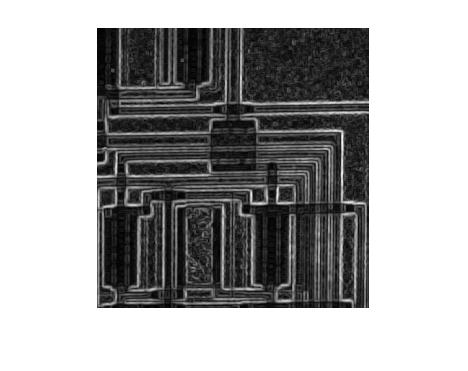
\includegraphics[width=\textwidth]{img/Fundamentacao/stdfilt_std}
%     \caption{Resultado da filtragem pelo filtro \textit{Desvio Padrão Local}}\label{fig:stdfilt:std}
%   \end{minipage}
%   \hfill
%   \begin{minipage}[b]{0.4\textwidth}
%     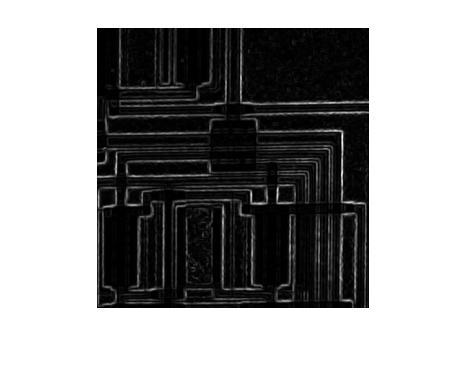
\includegraphics[width=\textwidth]{img/Fundamentacao/stdfilt_var}
%     \caption{Resultado da filtragem pelo filtro \textit{Variância Local}}\label{fig:stdfilt:var}
%   \end{minipage}
% \end{figure}

\FloatBarrier

\subsection{Método \textit{Otsu}}\label{sec:dom_esp:otsu}

\par Método \textit{Otsu} é um algoritmo usado para encontrar um limiar que melhor separa duas classes em um histograma \cite{otsumethod}.

\par O cálculo é feito de forma que a variância dentro da mesma classe é mínima e, consequentemente, a variância entre as classes é máxima. As \refEqs{eq:otsu:1}{eq:otsu:5} demonstram matemáticamente os cálculos feitos em cada etapa do algoritmo. Nas equações, $\{0, 1, 2, ..., L - 1\}$ são todos os \textit{L} possíveis valores do histograma, $p_{i}$ as probabilidades em que esses valores aparecem e \textit{t} o limiar sendo considerado para os cálculos. O limiar \textit{T} vai ser algum valor no intervalo $0 < T < L - 1$. As etapas do algoritmo são descritas abaixo:

\begin{enumerate}
    \item Calcular o histograma e as probablidades de cada valor do histograma;
    \item 
        Para cada $t = 0 \text{ até } L-1$:
        \begin{enumerate}
            \item Atualizar as probabilidades e as médias de cada classe;
            \item Calcular a variância entre as classes;
        \end{enumerate}
    \item Escolher o limiar \textit{T} de forma que seja a maior variância calculada.
\end{enumerate}

\equacao{eq:otsu:1}{\omega_{1}(t) = \sum_{i=0}^{t-1}p(i)}

\equacao{eq:otsu:2}{\omega_{2}(t) = \sum_{i=t}^{L-1}p(i)}

\equacao{eq:otsu:3}{\sigma_{b}^{2}(t) = \omega_{1}(t)\omega_{2}(t)(\mu_{1} - \mu_{2})^2}

\equacao{eq:otsu:4}{\mu_{1}(t) = \frac{1}{\omega_{1}(t)}\sum_{i=0}^{t-1}ip(i)}

\equacao{eq:otsu:5}{\mu_{2}(t) = \frac{1}{\omega_{2}(t)}\sum_{i=t}^{L-1}ip(i)}

\noindent onde $\omega_{1}(t)$ e $\omega_{2}(t)$ são as probabilidades de cada classe; $\sigma_{b}^{2}(t)$ a variância entre as duas classes; e $\mu_{1}(t)$ e $\mu_{2}(t)$ as médias das classes.

\par Sua principal aplicação é em processamento de imagens, e consiste em binarizar imagens em escala de cinza. A binarização é feita calculando o histograma da imagem e então encontrando o limiar (intensidade de \textit{pixel}) que melhor separa o fundo e o primeiro plano das imagens \cite{gonsalez2006}. A \refFig{fig:otsu} ilustra imagens antes e depois da binarização utilizando o método \textit{Otsu}.

\figurasDuplas{h!}{img/Fundamentacao/stdfilt_entrada}{img/Fundamentacao/otsu_binaria}{Processo de binarização de imagens utilizando o método \textit{Otsu}}{Imagem original}{Imagem binarizada}{fig:otsu}{fig:otsu:org}{{fig:otsu:bin}{.5\textwidth}{width=.5\textwidth}}

% \begin{figure}[h!]
% \centering
% \begin{subfigure}{.5\textwidth}
%   \centering
%   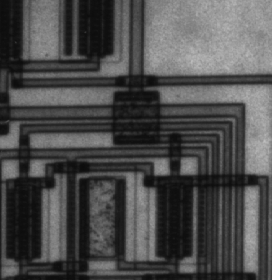
\includegraphics[width=.5\linewidth]{img/Fundamentacao/stdfilt_entrada.png}
%   \caption{Imagem antes da binarização.}
% \end{subfigure}%
% \begin{subfigure}{.5\textwidth}
%   \centering
%   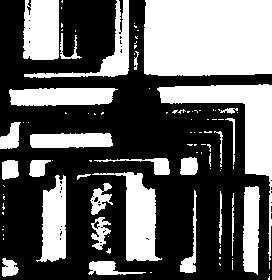
\includegraphics[width=.5\linewidth]{img/Fundamentacao/otsu_binaria.png}
%   \caption{Imagem binarizada.}
% \end{subfigure}
% \caption{Processo de binarização de imagens.}
% \label{fig:otsu}
% \end{figure}

\section{Processamento Morfológico de Imagens}\label{sec:morf}

\par Morfologia matemática é o estudo de estruturas geométricas. Operações morfológicas aplicadas em imagens consistem no processamento de regiões baseados em suas formas \cite{gonsalez2006}. 

\par A operação consiste em aplicar um elemento estruturante em uma imagem de entrada de forma a gerar uma imagem de saída. Os elementos estruturantes são matrizes e podem ter vários formatos e tamanhos, sendo círculos e quadrados os mais utilizados.

\par O elemento estruturante é sobreposto em todos os \textit{pixels} da imagem, de forma que todos os elementos com valor 1 no elemento são considerados na região sobreposta da imagem. Para todo elemento estrututante, é atribuído um \textit{ponto âncora}, que é o \textit{pixel} da região sobreposta da imagem de entrada processado. A \refFig{fig:kernel_morfo} ilustra um elemento estruturante.

\figura[!h]{img/Fundamentacao/kernel}{Exemplo de elemento estruturante. O elemento central sublinhado é o \textit{ponto âncora}}{fig:kernel_morfo}{width=0.3\textwidth}

\par Operações morfológicas são aplicadas em imagens geralmente para \cite{erosionDilationOpencv}:

\begin{itemize}
    \item Isolar elementos individuais;
    \item Juntar elementos que podem ser do mesmo objeto;
    \item Remover ruídos;
    \item Achar buracos ou sobreposições.
\end{itemize}

\par As duas principais operações morfológicas são a dilatação e erosão, e são explicadas nas Seções \ref{sec:morf:dil} e \ref{sec:morf:ero}, respectivamente.

\subsection{Dilatação} \label{sec:morf:dil}

\par Operação morfológica que aumenta regiões mais claras, ou diminui regiões mais escuras, da imagem de entrada \cite{gonsalez2006}. Pode ser utilizada também para calcular máximos locais de imagens.

\par O elemento estrututante é sobreposto em cada um dos \textit{pixels} da imagem de entrada, o máximo local da região sobreposta é calculado, e por fim, esse máximo é atribuído à imagem de saída na \textit{posição âncora} do elemento estruturante. A \refFig{fig:processo_dilatacao} ilustra as etapas descritas acima, considerando o elemento estrututante da \refFig{fig:kernel_morfo}.

\figura[!h]{img/Fundamentacao/dilatacao}{Resultado da etapa de dilatação. A matriz 3x3 centralizada corresponde ao elemento estrututante e o elemento sublinhado ao \textit{ponto âncora} substituído pelo máximo valor da região sobreposta}{fig:processo_dilatacao}{width=0.4\textwidth}

\par A \refFig{fig:dil} ilustra uma imagem de entrada para a operação de dilatação e a imagem de saída resultante, respectivamente.

\figuraBib[h!]{img/Fundamentacao/dil}{Imagem de entrada e saída da operação de dilatação}{erosionDilationOpencv}{fig:dil}{width=0.4\textwidth}%

\subsection{Erosão} \label{sec:morf:ero}

\par Operação morfológica que diminui regiões mais claras, ou aumenta regiões mais escuras, da imagem de entrada \cite{gonsalez2006}. Pode ser utilizada também para calcular mínimos locais de imagens.

\par Possui procedimentos parecidos com a operação de dilatação, mas ao invés de calcular os máximos das regiões sobrepostas pelo elemento estrututante, calcula os mínimos.

\par A \refFig{fig:ero} ilustra uma imagem de entrada para a operação de erosão e a imagem de saída resultante, respectivamente.

\figuraBib[!h]{img/Fundamentacao/ero}{Imagem de entrada e saída da operação de erosão}{erosionDilationOpencv}{fig:ero}{width=0.4\textwidth}%

%%%%%%%%%%%%%%%%%%%%%%%%%%%%%%%%%%%%%%%%%%%%%%%%%%%%%%%%%%%%%%%%%%%%%%%%%%%%%%%%
%%%%%%%%%%%%%%%%%%%%%%%%%%%%%%%%%%%%%%%%%%%%%%%%%%%%%%%%%%%%%%%%%%%%%%%%%%%%%%%%
%%%%%%%%%%%%%%%%%%%%%%%%%%%%%%%%%%%%%%%%%%%%%%%%%%%%%%%%%%%%%%%%%%%%%%%%%%%%%%%%
\section{Filtragem de Imagens} \label{sec:fundamentacao:filtragem}

\par Filtros são processos que modificam sinais de entrada. Como imagens são sinais, o processo de filtrar imagens consiste em modificá-las \cite{gonsalez2006}. Filtros podem ser usados para remover componentes indesejados, realçar componentes desejados ou até para extrair informações ou atributos do sinais sendo processados \cite{loggabor-kovesi}.

\par Imagens podem ser filtradas tanto no domínio do espaço quanto da frequência. A filtragem no domínio espacial consiste em realizar o processo de convolução \textit{2D} por meio de filtros espaciais, chamados de máscaras ou \textit{kernel}\cite{oppenheim2013signals}. A convolução \textit{2D} pode ser representada matemáticamente pela equação

\equacao{eq:filtragem:convolucao}{g(x,y) = \sum_{s=-a}^{a}\Bigg(\sum_{t=-b}^{b}H(s,t)I(x-s,y-t)\Bigg)}

\noindent onde $g$ é a convolução, $H$ o \textit{kernel} e $I$ a imagem sendo filtrada\cite{gonsalez2006}. A equação

\equacao{eq:filtragem:convolucao_simplificada}{g = I*H}

\noindent é a versão simplificada da \refEq{eq:filtragem:convolucao}.

\par Já a filtragem no domínio da frequência, consiste apenas na multiplicação da imagem e do \textit{kernel} transformados para o domínio da frequência pela \textit{Transformada de Fourier} (\textit{F(.)}) \cite{gonsalez2006}. A equação

\equacao{eq:filtragem:relacao}{I*H \iff F(I) \cdot F(H)}

\noindent ilustra a relação entre as filtragens nos dois espaços.

\par Filtragem no domínio da frequência é útil quando deseja-se remover ou realçar um intervalo de frequências da imagem.

\subsection{\textit{Filtro Log-Gabor}}\label{sec:fundamentacao:filtragem:loggabor}

\par O filtro \textit{Log-Gabor} é uma adaptação do filtro \textit{Gabor}, mas na escala logarítmica, e é um filtro linear passa banda \cite{field1987-loggabor, masek2003}. Possui duas características que o diferem: não possui componentes \textit{DC} e não pode ser representado por uma máscara no domínio do espaço, de forma que é exclusivo ao domínio da frequência \cite{loggabor-kovesi}. Assim como o filtro \textit{Gabor}, é muito utilizado para a extração de atributos e codificação de íris \cite{masek2003}.

\par A função de ativação do filtro \textit{Log-Gabor} é representada pela equação

\equacao{eq:filtragem:loggabor}{H(\omega) = e^{\frac{-log(\omega/\omega_{0})^{2}}{2log(\sigma)^{2}}}}

\noindent  onde $\sigma$ controla a largura de banda e $\omega_{0}$ a frequência central do filtro. Já a \refFig{fig:loggabor}, ilustra a função de ativação do filtro na escala linear.

\figura[!h]{img/Fundamentacao/loggabor}{Função de ativação do filtro \textit{Log-Gabor} na escala linear}{fig:loggabor}{width=0.5\textwidth}


%%%%%%%%%%%%%%%%%%%%%%%%%%%%%%%%%%%%%%%%%%%%%%%%%%%%%%%%%%%%%%%%%%%%%%%%%%%%%%%%
%%%%%%%%%%%%%%%%%%%%%%%%%%%%%%%%%%%%%%%%%%%%%%%%%%%%%%%%%%%%%%%%%%%%%%%%%%%%%%%%
%%%%%%%%%%%%%%%%%%%%%%%%%%%%%%%%%%%%%%%%%%%%%%%%%%%%%%%%%%%%%%%%%%%%%%%%%%%%%%%%

\section{Sistemas Biométricos de Íris}

\par Sistemas biométricos de íris são sistemas que utilizam algoritmos de reconhecimento de íris para autenticação biométrica. Íris possuem inúmeras vantagens e desvantagens para seu uso, como listadas abaixo \cite{advantagesDaugman}:

\par Vantagens: 

\begin{itemize}
    \item Órgão protegido;
    \item Padrões possuem alta distintividade;
    \item Padrões são imutáveis ao longo da vida;
    \item A velocidade de processamento do módulo de \textit{decisão} é rápida.
\end{itemize}

\par Desvantagens:

\begin{itemize}
    \item Precisa ser capturada em distâncias pequenas;
    \item Olho em movimento atrapalha a etapa de segmentação;
    \item Cílios, pálpebras e reflexos atrapalham a etapa de segmentação;
    \item A dilatação da pupila pode eliminar alguns padrões da íris.
\end{itemize}

\par A Seção \ref{sec:iris:olho} explica o que é a íris e suas funções; a Seção \ref{sec:iris:nir_vl} explica as diferenças, as vantagens e desvantagens do uso de imagens de olho \textit{\acrfull{NIR}} e \textit{\acrfull{LV}} em sistemas de reconhecimento de íris; e por fim, a Seção \ref{sec:iris:rec_iris} explica como algoritmos de reconhecimento de íris funcionam.

\subsection{Olho humano}\label{sec:iris:olho}

\par Íris é um órgão do globo ocular e é caracterizada por ser a parte circular colorida e pigmentada do olho humano \cite{irisDaugman}. Possui músculos que, ao contrair e dilatar a pupila, controlam a quantidade de luz que entra na retina \cite{adlerIris2003}. A \refFig{fig:olhohumano} ilustra a íris, pupila, retina e as outras estruturas do olho humano.

\figuraBib[!h]{img/Fundamentacao/olho-humano}{Anatomia de um olho humano}{imgOlhoHumano}{fig:olhohumano}{width=0.4\textwidth}%

\par A íris apresenta alta variedade de padrões e colorações, que podem variar do azul, castanho, verde, avelã até o cinza. A cor da íris é definida geneticamente, enquanto os padrões não \cite{adlerIris2003}. A íris do olho esquerdo de um indivíduo é necessariamente diferente da do olho direito \cite{wayman2005biometric}. Essa diferença é ilustrada nas \refFigs{fig:iris_direita}{fig:iris_esquerda}.

\par Com a probabilidade de 1 em $10^{72}$ de existirem padrões de íris iguais e não modificarem ao longo da vida, é considerada um dos melhores tipos de biometria \cite{iris_UFRJ}.

\figurasDuplas{h!}{img/Fundamentacao/iris_direita}{img/Fundamentacao/iris_esquerda}{Diferança das íris do olho humano (Fonte: \cite{trokielwicz2016-Warsaw})}{Íris do olho direito}{íris do olho esquerdo}{fig:olhos}{fig:iris_direita}{{fig:iris_esquerda}{.5\textwidth}{width=.5\textwidth}}

% \begin{figure}[h!]
% \centering
% \begin{subfigure}{.5\textwidth}
%   \centering
%   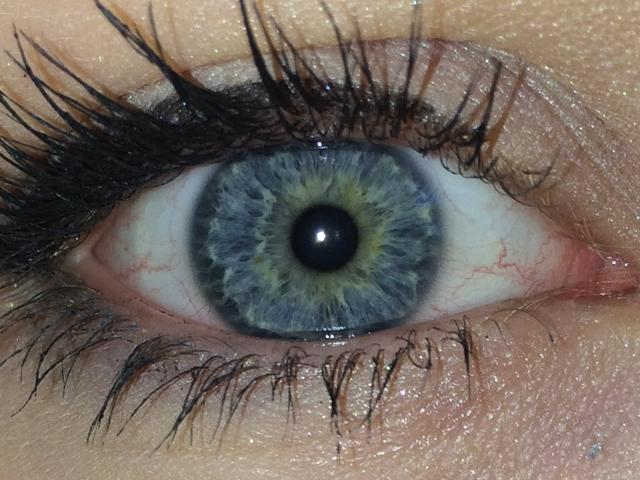
\includegraphics[width=.5\linewidth]{img/Fundamentacao/iris_direita}
%   \caption{Íris do olho direito.}\label{fig:iris_direita}
% \end{subfigure}%
% \begin{subfigure}{.5\textwidth}
%   \centering
%   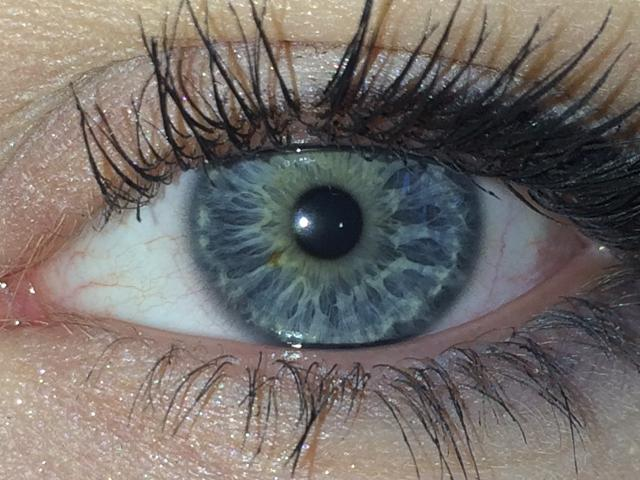
\includegraphics[width=.5\linewidth]{img/Fundamentacao/iris_esquerda}
%   \caption{Íris do olho esquerdo.}\label{fig:iris_esquerda}
% \end{subfigure}
% \caption{Diferença das íris do olho humano.}
% \label{fig:olhos}
% \end{figure}

% \begin{figure}[!h]
%   \centering
%   \begin{minipage}[b]{0.4\textwidth}
%     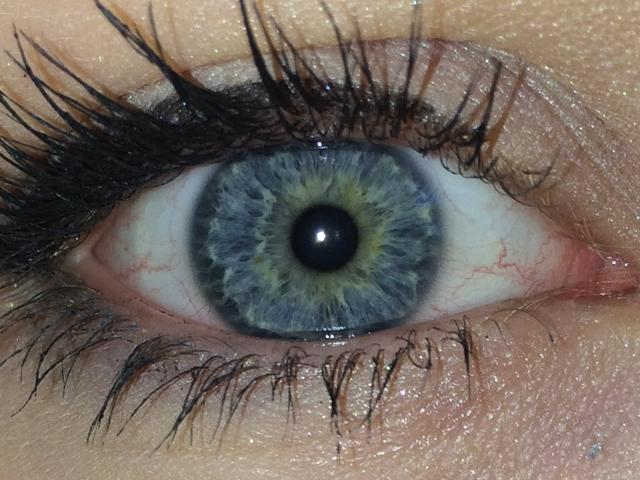
\includegraphics[width=\textwidth]{img/Fundamentacao/iris_direita.jpg}
%     \caption{Íris do olho direito.}\label{fig:iris_direita}
%   \end{minipage}
%   \hfill
%   \begin{minipage}[b]{0.4\textwidth}
%     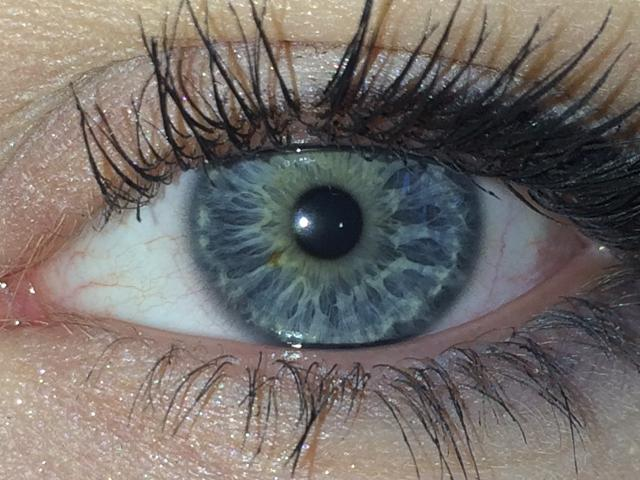
\includegraphics[width=\textwidth]{img/Fundamentacao/iris_esquerda.jpg}
%     \caption{Íris do olho esquerdo.}\label{fig:iris_esquerda}
%   \end{minipage}
% \end{figure}

\subsection{\textit{Imagens \acrfull{LV} vs \acrfull{NIR}}} \label{sec:iris:nir_vl}

\par Espectro eletromagnético é o intervalo de ondas que são caracterizadas por comprimento de onda, frequência e energia \cite{gonsalez2006}. A \refFig{fig:espectro} ilustra o espectro de ondas eletromagnéticas.

\figuraBib[!h]{img/Fundamentacao/espectro_eletromagnetico}{Espectro de ondas eletromagnéticas}{espectroeletromagnetico}{fig:espectro}{width=0.5\textwidth}%

Imagens \textit{\arcshort{LV}} são imagens capturadas por aparelhos, como câmeras fotográficas comuns, que possuem comprimento de onda no intervalo 430-790 \textit{nm} no espectro eletromagnético, e é o intervalo perceptível pelo olho humano \cite{gonsalez2006}.

\par Já imagens \arcshort{NIR} são imagens que possuem comprimento de onda no intervalo 800-900 \textit{nm} no espectro eletromagnético \cite{gonsalez2006}. O olho humano não é capaz de perceber esse intervalo no espectro eletromagnético, mas câmeras fotográficas especiais são capazes de capturá-las e registrá-las, de forma que possibilitam o estudo de suas propriedades\cite{nir}.


\par Imagens \textit{\arcshort{LV}} de íris ilustram todas as suas possíveis variações de cores, citadas na Seção \ref{sec:iris:olho}. Porém, alguns dos padrões da íris acabam sendo perdidos ou tendo qualidade ruim, especialmente de íris de cores mais escuras, já que os padrões também apresentam coloração escura. Imagens de íris \arcshort{NIR} diminuem o efeito dos reflexos e da perda de padrões em imagens de íris escuras, além de destacarem os padrões da íris \cite{abdullah2015}. Por conta dessas propriedades, imagens \arcshort{NIR} são as mais utilizadas em sistemas de reconhecimento de íris \cite{daugman2004}. As \refFigs{fig:pigmentacoes}{fig:iris_nir} ilustram imagens de íris \textit{\arcshort{LV}} com pigmentação escura e clara, e imagem de íris \textit{\arcshort{NIR}}, respectivamente.

\figurasDuplas{ht!}{img/Fundamentacao/iris_vl_escura}{img/Fundamentacao/iris_vl_clara}{Imagens de íris \textit{\acrshort{LV}} (Fonte: \cite{trokielwicz2016-Warsaw})}{Pigmentação escura)}{Pigmentação clara}{fig:pigmentacoes}{fig:iris_vl_escura}{{fig:iris_vl_clara}{.5\textwidth}{width=.6\linewidth}}

\figuraBib[ht!]{img/Fundamentacao/iris_nir_daugman}{Imagem de íris \textit{\arcshort{NIR}}}{nirDaugman}{fig:iris_nir}{width=0.3\textwidth}%

\subsection{Reconhecimento de íris} \label{sec:iris:rec_iris}

\par Algoritmos de reconhecimento de íris são algoritmos que implementam técnicas de segmentação, codificação e correspondência para identificar indivíduos usando suas íris \cite{wayman2005biometric, daugman2004}.

\par Como explicado na Seção \ref{sec:sis_bio:processamento}, o módulo de \textit{processamento} de um sistema biométrico consiste em duas etapas: segmentar e extrair os atributos da característica biométrica. 

\par Algoritmos de segmentação de íris consistem, geralmente, na implementação dos seguintes passos \cite{daugman2004, masek2003}:

\begin{enumerate}
    \item Encontrar os raios e a posições do centro da íris e da pupila;
    \item Normalizar a íris.
\end{enumerate}

\par A maioria dos algoritmos de segmentação utilizam para encontrar as posições centrais e os raios da íris e pupila o \textit{Operador Integro-Diferencial} \cite{daugman2004}. O operador consiste em uma fórmula que detecta as bordas circulares e é usado separadamente para a íris e a pupila. O \textit{Operador Integro-Diferencial} é descrito pela equação

\equacao{eq:rec_iris:integro-differential}{
    max_{(r,x_{0},y_{0})}\Big|G_{\sigma}(r)*\frac{\partial}{\partial r}\oint_{r,x_{0},y_{0}}\frac{I(x,y)}{2 \pi r}ds\Big|
}

\noindent e é aplicado por toda a imagem até que um formato circular é encontrado, onde $I(x,y$) é a imagem com um olho humano, $2\pi r$ o contorno da imagem, $r$ e $(x_{0}, y_{0})$ o raio e a posição do central da imagem inicialmente e $G_{\sigma}$ é um filtro \textit{Gaussiano} usado para suavizar ruídos.

\par O passo de normalização é feito de forma a transformar a imagem da íris segmentada para dimensões fixas e para a extração dos atributos, e geralmente consiste na utilização do \textit{Modelo Rubber Sheet} \cite{daugman2004}. Esse modelo transforma a imagem da íris segmentada das coordenadas cartesianas para polares $(x,y) \mapsto (\rho,\theta)$. A \refFig{fig:rubber_sheet} ilustra o procedimento realizado pelo \textit{Modelo Rubber Sheet} e a \refFig{fig:normalizada} uma imagem de íris normalizada com esse modelo. Nessa etapa, uma máscara binária da imagem normalizada também é gerada, de forma a separar íris de ruídos e ser utilizada no módulo de \textit{decisão}.

\figuraBib[h!]{img/Fundamentacao/rubber_sheet}{Procedimento do \textit{Modelo Rubber Sheet}}{rubberSheet}{fig:rubber_sheet}{width=0.4\textwidth}

\figurasDuplas{h!}{img/Fundamentacao/iris_original_normalizada}{img/Fundamentacao/iris_normalizada}{Processo de normalização de uma imagem de íris segmentada}{Imagem original antes da normalização}{Imagem de íris normalizada}{fig:normalizacao}{fig:antes_normalizada}{{fig:normalizada}{.5\textwidth}{width=.8\linewidth}}

\par A extração de atributos em reconhecimento de íris recebe o nome de codificação \cite{daugman2004}. A etapa de codificação consiste, geralmente, na aplicação das \textit{Wavelets 2D de Gabor} na imagem da íris normalizada, de forma a gerar um código de íris (\textit{IrisCode}) único, que é o modelo ou \textit{template} da característica biométrica \cite{daugman2006}. \textit{Wavelets 2D de Gabor} extraem atributos da íris como uma sequência de vetores com números \textit{complexos} e então usa os ângulos de suas fases para quantizar uma sequência de dois \textit{bits} dependendo do quadrante no plano \textit{complexo}, conforme a \refFig{fig:phase_modulator} \cite{daugman2004}. São extraídos no total do processo, 2048 \textit{bits} (256 \textit{bytes}) \cite{daugman2004}. A \refFig{fig:iriscode} ilustra uma imagem de íris segmentada com o seu \textit{IrisCode}.

\figuraBib[ht!]{img/Fundamentacao/phase_modulator}{Codificação pelos quadrantes do plano \textit{complexo} das \textit{Wavelets 2D de Gabor}}{daugman2004}{fig:phase_modulator}{width=.3\textwidth}

\figuraBib[ht!]{img/Fundamentacao/iriscode}{Imagem segmentada e seu \textit{IrisCode} gerado}{irisCode}{fig:iriscode}{width=.4\textwidth}

\par As \textit{Wavelets 2D de Gabor} são calculadas pela equação
\equacao{eq:rec_iris:2d-gabor-wavelet}{
    h\{Re,Im\} = sgn_{\{Re, Im\}}\int_{\rho}\int_{\phi}I(\rho,\phi)e^{-i\omega(\theta_{0}-\phi)}\cdot e^{-(r_{0}-\rho)^2/\alpha^2}e^{-(\theta_{0}-\phi)^2/\beta^2}\rho d \rho d\phi
}

\noindent onde $h\{Re,Im\}$ é um valor complexo em que tanto a parte real quanto imaginária pode ser 0 ou 1, dependendo do sinal (\textit{sgn}) da integral; $I(\rho,\phi)$ é a imagem da íris normalizada nas coordenadas polares; $\alpha$ e $\beta$ são parâmetros de tamanho da \textit{wavelet 2D}; $\omega$ a frequência da \textit{wavelet}; e por fim, $r_{0}$ e $\theta_{0}$ são as coordenadas da imagem da íris na coordenada polar sendo calculadas.

\par Na Seção \ref{sec:sis_bio:decisao}, o módulo de \textit{decisão} de um sistema biométrico é explicado e consiste no cálculo da diferença ou similaridade de dois \textit{templates} gerados no módulo de \textit{processamento} de forma a verificar se há ou não correspondência entre eles.

\par Em reconhecimento de íris, essa comparação é feita, geralmente, pelo cálculo da diferença entre os \textit{IrisCodes} e as máscaras binárias das imagens normalizadas pela \textit{\acrfull{HD}} fracional \cite{daugman2004}.



\par O cálculo da \textit{\acrshort{HD}} é feito pela equação

\equacao{eq:HD}{
    HD = \frac{\|(códigoA \otimes códigoB) \cap máscaraA \cap máscaraB\|}{\|máscaraA \cap máscaraB\|},
}

\noindent onde \textit{código} e \textit{máscara} A e B são os códigos e máscaras sendo comparadas; $\otimes$ e $\cap$ são as operações \textit{booleanas} \textit{XOR} e \textit{AND}; e $\| \|$ são as normas dos vetores de \textit{bits}. O resultado dessa equação são valores entre 0 e 1, onde 0 é uma correspondência perfeita \cite{daugman2004}.

% \begin{figure}[h!]
% \centering
% \begin{subfigure}{.5\textwidth}
%   \centering
%   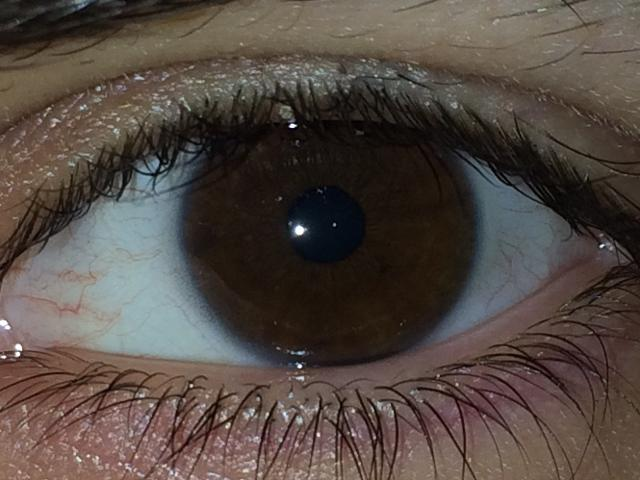
\includegraphics[width=.5\linewidth]{img/Fundamentacao/iris_vl_escura}
%   \caption{Pigmentação escura.}\label{fig:iris_vl_escura}
% \end{subfigure}%
% \begin{subfigure}{.5\textwidth}
%   \centering
%   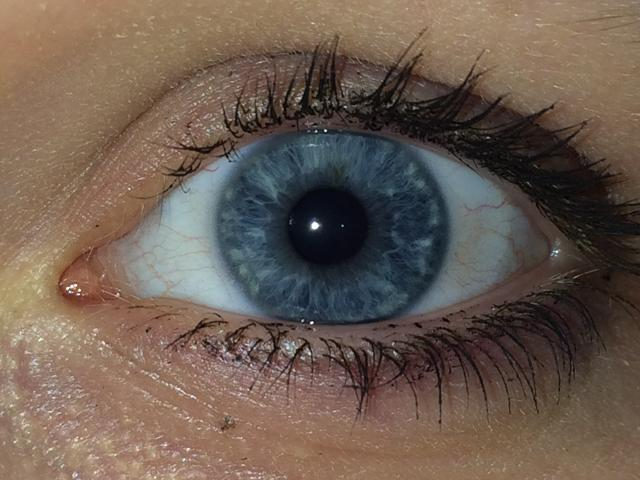
\includegraphics[width=.5\linewidth]{img/Fundamentacao/iris_vl_clara}
%   \caption{Pigmentação clara.}\label{fig:iris_vl_clara}
% \end{subfigure}
% \caption{Imagens de íris \textit{\acrshort{LV}}.}
% \label{fig:pigmentacoes}
% \end{figure}

% \begin{figure}[h!]
%   \centering
%   \begin{minipage}[b]{0.4\textwidth}
%     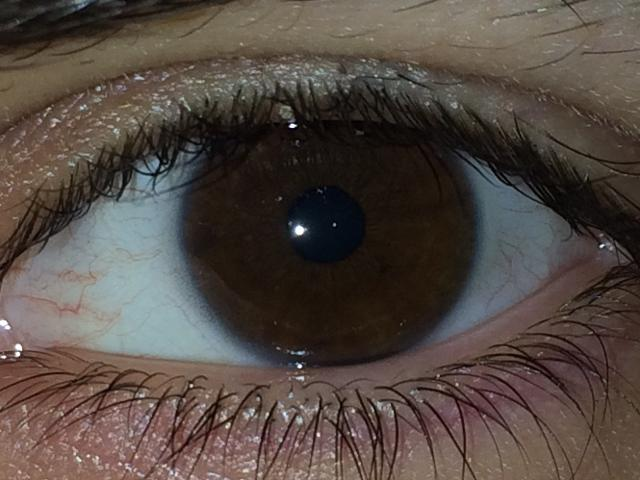
\includegraphics[width=\textwidth]{img/Fundamentacao/iris_vl_escura.jpg}
%     \caption{Imagem de íris \textit{\arcshort{LV}} com pigmentação escura.} \label{fig:iris_vl_escura}
%   \end{minipage}
%   \hfill
%   \begin{minipage}[b]{0.4\textwidth}
%     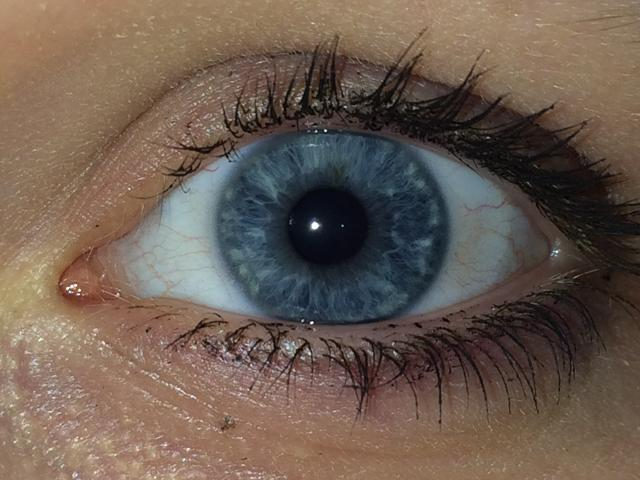
\includegraphics[width=\textwidth]{img/Fundamentacao/iris_vl_clara.jpg}
%     \caption{Imagem de íris \textit{\arcshort{LV}} com pigmentação clara.}\label{fig:iris_vl_clara}
%   \end{minipage}
% \end{figure}

\par No próximo capítulo é realizada uma revisão de artigos que implementaram métricas de qualidade de imagem e é explicado com mais detalhes as métricas de qualidade escolhidas para a implementação deste projeto: \textit{\acrfull{DSMI}} e \textit{\acrfull{FCE}}.